\section{Программное обеспечение}\label{sec:secSoft}

Программное обеспечение системы считывания и сбора данных прототипа CBM~RICH представляет собой набор модулей приема, первичной обработки и сохранения данных, реализованных в рамках программного каркаса CbmRoot~\cite{CBMROOT}. CbmRoot вместе в FLESnet~\cite{FLESnet} образуют инфраструктуру, позволяющую выполнять приём данных, моделирование, реконструкцию и анализ данных эксперимента CBM.

Соответствующим образом сконфигурированное приложение, написанное в рамках CbmRoot, может быть запущено на ЭВМ, как частный случай на распределённой вычислительной системе. Все этапы от считывания до анализа могут быть выполнены ``на лету'', без записи промежуточных результатов на диск. В ходе описываемых в данной статье тестов использовалась последовательность обработки данных, изображённая на \figref{fig:SoftDiag}. Программная реализация, функционал и взаимодействие отдельных блоков описаны ниже.

\begin{figure}[H]
\centering
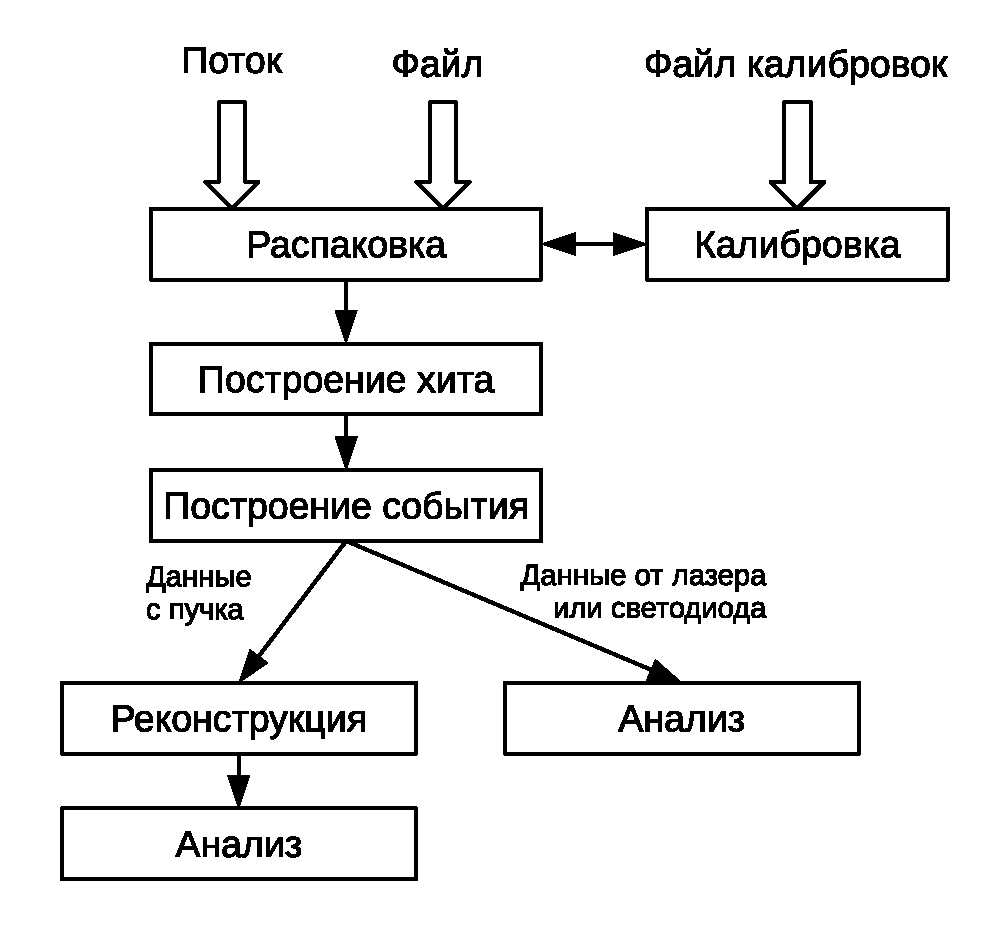
\includegraphics[width=0.6\textwidth]{pictures/13_Software_diagram.eps}
\caption{Диаграмма взаимодействия программных модулей.}
\label{fig:SoftDiag}
\end{figure}

%(Напишите об особенностях софта для работы с данными в случае использования FLIB.)
%\textbf{
%Все описанные ниже этапы обработки применимы как к данным с TRB~v3, как они есть сейчас, так и с FLIB в финальной конфигурации. Принципиальным отличием является то, что FLIB оперирует не DAQ-событиями, а срезами времени (см.~\ref{sec:secFinalReadout}) и интервалами. Интервал представляет собой пакет данных, содержащий информацию с нескольких детекторов за ограниченный промежуток времени. Для того, чтобы получить интервал, необходимо выполнить так называемое ``построение интервала''~\cite{}, которое осуществляется FLESnet на вычислительных узлах FLES.
%}
%(В общем, я не вижу смысла тут углубляться, особенно учитывая, что я не так хорошо знаю эту тему. Суть в том, что в софте практически ничего не меняется. В том, что я описываю, вообще ничего не меняется. Все особенности --- они ещё до распаковки.
%Можно представить это так:
%Если есть один только рич прототип, то я даже не могу так сказать, в чём отличие DAQ-события от среза времени и от интервала. Например один TRB типа концентратор, собрав всё с нескольких FEB'ов формирует один поток DAQ-событий. Каждое DAQ-событие содержит все хиты за период синхро-генератора. Это же по определению срез времени. А так как поток один, то это же и интервал.
%Если, скажем, у рича очень много каналов и невозможно уместить всё в один флиб-линк чисто из-за пропускной способности, или есть несколько логически разных потоков данных, то есть с двух или более детекторов, то нужно выполнять построение интервала. Этим занимается FLESnet, который и предоставляет CbmRoot'у данные в таком виде, что можно забыть о том, с FLIB'а они или TRB.)

%Вот новый постер о FLES этого года.
%Сделать ссылку
%https://indico.cern.ch/event/505613/contributions/2227522/attachments/1346746/2039013/Poster-v1-317.pdf

\subsection{Распаковка}\label{sec:secUnpacking}

Распаковка --- это первый этап обработки данных, поступающих с электроники. В CbmRoot есть возможность обрабатывать данные как поступающие напрямую с детекторов, так и сохранённые в файле (с помощью DABC в формате HLD --- HADES list mode data format~\cite{HLD}). При использовании FLIB распаковке предшествует запуск небольшого интерфейсного модуля, который выделяет из поступающего от FLESnet потока данных в формате временных интервалов (TSA --- Time Slice Archive), сообщения, относящиеся к детектору RICH. Распаковка реализована как task-класс \classname{CbmRichTrbUnpack}. В результате выполнения каждой итерации на выходе формируется \classname{TClonesArray} с объектами класса \classname{CbmTrbRawMessage}.

\subsection{Калибровка точного времени}\label{sec:secSoftFineTimeCalib}

В процедуре калибровки точного времени воплощена известная техника калибровки счётчика цифровой линии задержки, реализованного с помощью технологии Tapped delay line \cite{TDLCALIB}, основанная на том, что распределение времен прихода сигналов должно быть равномерным по временному интервалу, занимаемому всеми элементами задержки. В результате анализа набранной порции данных для каждого канала строится дискретная функция $ f_{calib}(Fine) $, называемая таблицей перехода от значения счётчика к значению точного времени в наносекундах. При использовании таблицы калибровки точного времени полное время вычисляется как $ T = Epoch \cdot 2048 \cdot 5 + Coarse \cdot 5 - f_{calib}(Fine) $~нс.

Процедура калибровки точного времени реализована в singleton-классе \classname{CbmTrbCalibrator}, который не является частью конвейера обработки данных --- обращение к объекту данного класса может производиться из любого места в программе. Присутствует возможность сохранения таблиц калибровки в отдельном файле, что ускоряет многократные расчёты за счёт повторного использования однократно рассчитанных таблиц.

\subsection{Коррекция задержек между каналами}\label{sec:secSoftDelayCorr}

Для коррекции задержек между каналами в классе \classname{CbmTrbCalibrator} реализована возможность импорта таблицы коррекций, построенной предварительно с помощью CmbRoot-макросов ``ExtractDelays'' и ``BuildDeltaTable'' на основе результатов первого прогона анализа. Первый макрос извлекает параметры гистограмм в текстовом виде из многочисленных файлов результатов анализа, полученных с помощью CbmRoot, возможно, с применением параллельных расчётов. Второй макрос стоит таблицу коррекций по данным параметрам.

Алгоритм коррекции задержек состоит в следующем. Введём сплошную нумерацию пикселей по всей фоточувствительной камере, состоящей из множества МА~ФЭУ. Полное число пикселей $ M = 64 \cdot N $, где $N$ --- число МА~ФЭУ. Для анализа отбираются все передние фронты, имеющие временную отметку, попадающую в заданное временное окно относительно триггера срабатывания лазера. Ширина и положение окна зависят от экспериментальной установки (например, разницы длин кабелей, точности регистрации триггера) и характеристик лазера и подбираются в соответствии с распределением, построенным по конкретному набору данных. Обычно ширина составляет около 100~нс, а левая граница сдвинута от триггера на 20~нс. По всему массиву отобранных данных строятся гистограммы разности временных отметок i-го и j-го каналов, где i~и~j пробегают значения от 1~до~$M$. В качестве меры разности задержек между каналами можно взять по выбору пользователя либо среднее значение распределения, либо наиболее вероятное. Полученные значения заполняют кососимметричную матрицу $A$ размерности $ M \cdot M $. В дальнейшем пользователь может задать опорный канал, относительно которого будет создана таблица коррекций, являющаяся, по сути, столбцом матрицы~$A$.

\subsection{Построение хита}\label{sec:secHitBuilding}

Сигнал от каждого зарегистрированного фотона, называемый хитом, состоит из двух сообщений, содержащих временные отметки переднего и заднего фронтов. Т.к.~разные каналы имеют разные задержки и вероятность регистрации отдельных фронтов не равна~100\%, необходимо было в анализе данных реализовать алгоритм подбора пар фронтов. Данная процедура реализована в task-классе \classname{CbmTrbEdgeMatcher}, который стоит в конвейере после распаковки и фактически выполняется после применения всех калибровок.

Для каждого входного канала был реализован буфер сообщений, который наполнялся передними фронтами по мере их поступления. Далее, как только приходил задний фронт, из буфера выбирался наиболее близкий по временной отметке передний фронт внутри заданного допустимого временного окна. На \figref{fig:EdgeMatching} приведён пример буфера передних фронтов для заданной пары каналов ВЦП в момент прихода одного заднего фронта. Время над порогом~(ToT) --- параметр хита, говорящий об амплитуде сигнала. Он вычисляется как разница временных отметок заднего и переднего фронтов в подобранной паре. Допускаются как положительные, так и отрицательные значения~ToT, однако в обе стороны накладывается ограничение.

\begin{figure}[H]
\centering
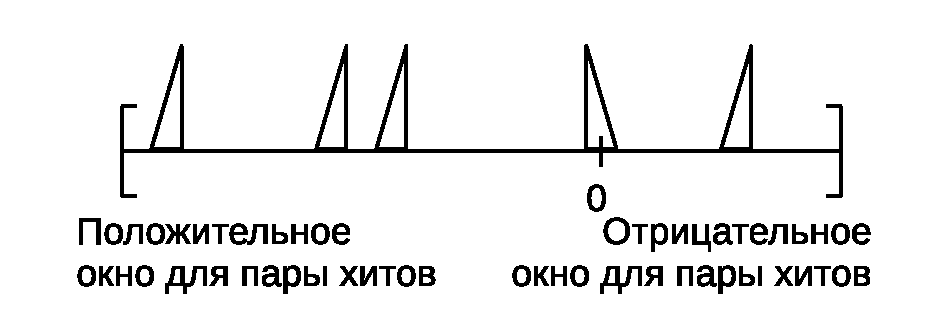
\includegraphics[width=0.6\textwidth]{pictures/14_Edge_matching_rus.eps}
\caption{Постановка задачи поиска пар фронтов для одного входного канала.}
\label{fig:EdgeMatching}
\end{figure}

Т.к.~не всегда присутствует соответствующий парный (передний либо задний) фронт, буфер постепенно наполняется и его необходимо очищать, чтобы избежать переполнения. Если для поступившего заднего фронта нет кандидата переднего фронта в буфере это означает, что передний фронт не был зарегистрирован. В таком случае этот задний фронт отбрасывается. Количество ненайденных фронтов сильно зависит от нагруженности входного канала, которая в свою очередь зависит от порога дискриминатора. При низком пороге регистрируется высокочастотный шум электроники, что приводит к формированию огромного потока выходных сообщений, которые не могут быть переданы из-за ограниченной пропускной способности выходного тракта системы считывания.

Предусмотрена возможность допускать одиночные передние фронты в качестве хитов, однако практика показала, что в этом нет смысла, т.к. в нормальном режиме ненайденные пары в основном обусловлены ошибками ВПЦ и доля таких сообщений пренебрежимо мала --- менее $ 2 \cdot 10^{-4} $.

\subsection{Построение события}\label{sec:secEventBuilding}

Тот факт, что физическая программа эксперимента CBM подразумевает исследование очень редких явлений, для которых практически невозможно вырабатывать аппаратный триггер, привёл к решению разработать и использовать бестриггерную систему считывания. В бестриггерной системе считывания каждый канал передней электроники вырабатывает сообщение при преодолении входным аналоговым сигналом установленного порога. Получается, что электроника выдаёт для программного обеспечения непрерывный поток никак не сгруппированных сообщений, содержащих временную отметку. Для того, чтобы выполнять физический анализ, необходимо в этом непрерывном потоке выделять осмысленные группы, которые мы называем событиями. Строго говоря, задача построения событий --- это одномерная задача кластеризации на оси времени с последующим отбором кластеров по некоторым критериям.

Задача также усложнена тем фактом, что электроника не может обеспечить непрерывный поток сообщений, упорядоченных по времени регистрации. Происходит группировка сообщений в так называемые DAQ-события, которые необходимы для обеспечения передачи информации, а сообщения внутри DAQ-событий могут быть упорядочны произвольно. Соответственно первый этап построения события --- упорядочивание сообщений.

В данных с пучковых тестов 2014~г., для того, чтобы определить, является ли распознанная группа событием, можно использовать сигналы с детекторов пучка --- пороговых черенковских счётчиков, годоскопов и др. В лабораторных данных, где выполнялись измерения с лазером, в качестве триггера можно использовать сигнал от генератора, управляющего лазером. В ситуации, когда нет дополнительной информации, как в случае полного детектора RICH в итоговом эксперименте, необходимо принимать решение о том, является распознанная группа событием, или нет, на основе исключительно информации, полученной из этой группы. Распознанный кластер может являться событием, но чаще всего будет состоять из одного сообщения --- шумового хита. Следовательно можно использовать кол-во хитов в событии для подавления шумов, что особенно актуально для дететора CBM~RICH, где выполняется реконструкция черенковских колец, требующая некоторого минимального числа хитов в плоскости реконструкции.

(Сначала общая идея, что в любом случае будет некоторое временное окно и все сообщения попадающие в окно формируют событие. Размеры окна --- один из параметров построителя событий, которым можно играть с целью повышения эффективности.)

(А ниже описывается предлагаемый алгоритм)

В силу того, что электроника бестриггерная и приём данных осуществляется порциями, называемыми DAQ-событиями, никак не связанными с реальными событиями, для формирования корректной входной информации для реконструкции и дальнейшего анализа данных необходимо выполнять процедуру построения события.

\begin{figure}[H]
\centering
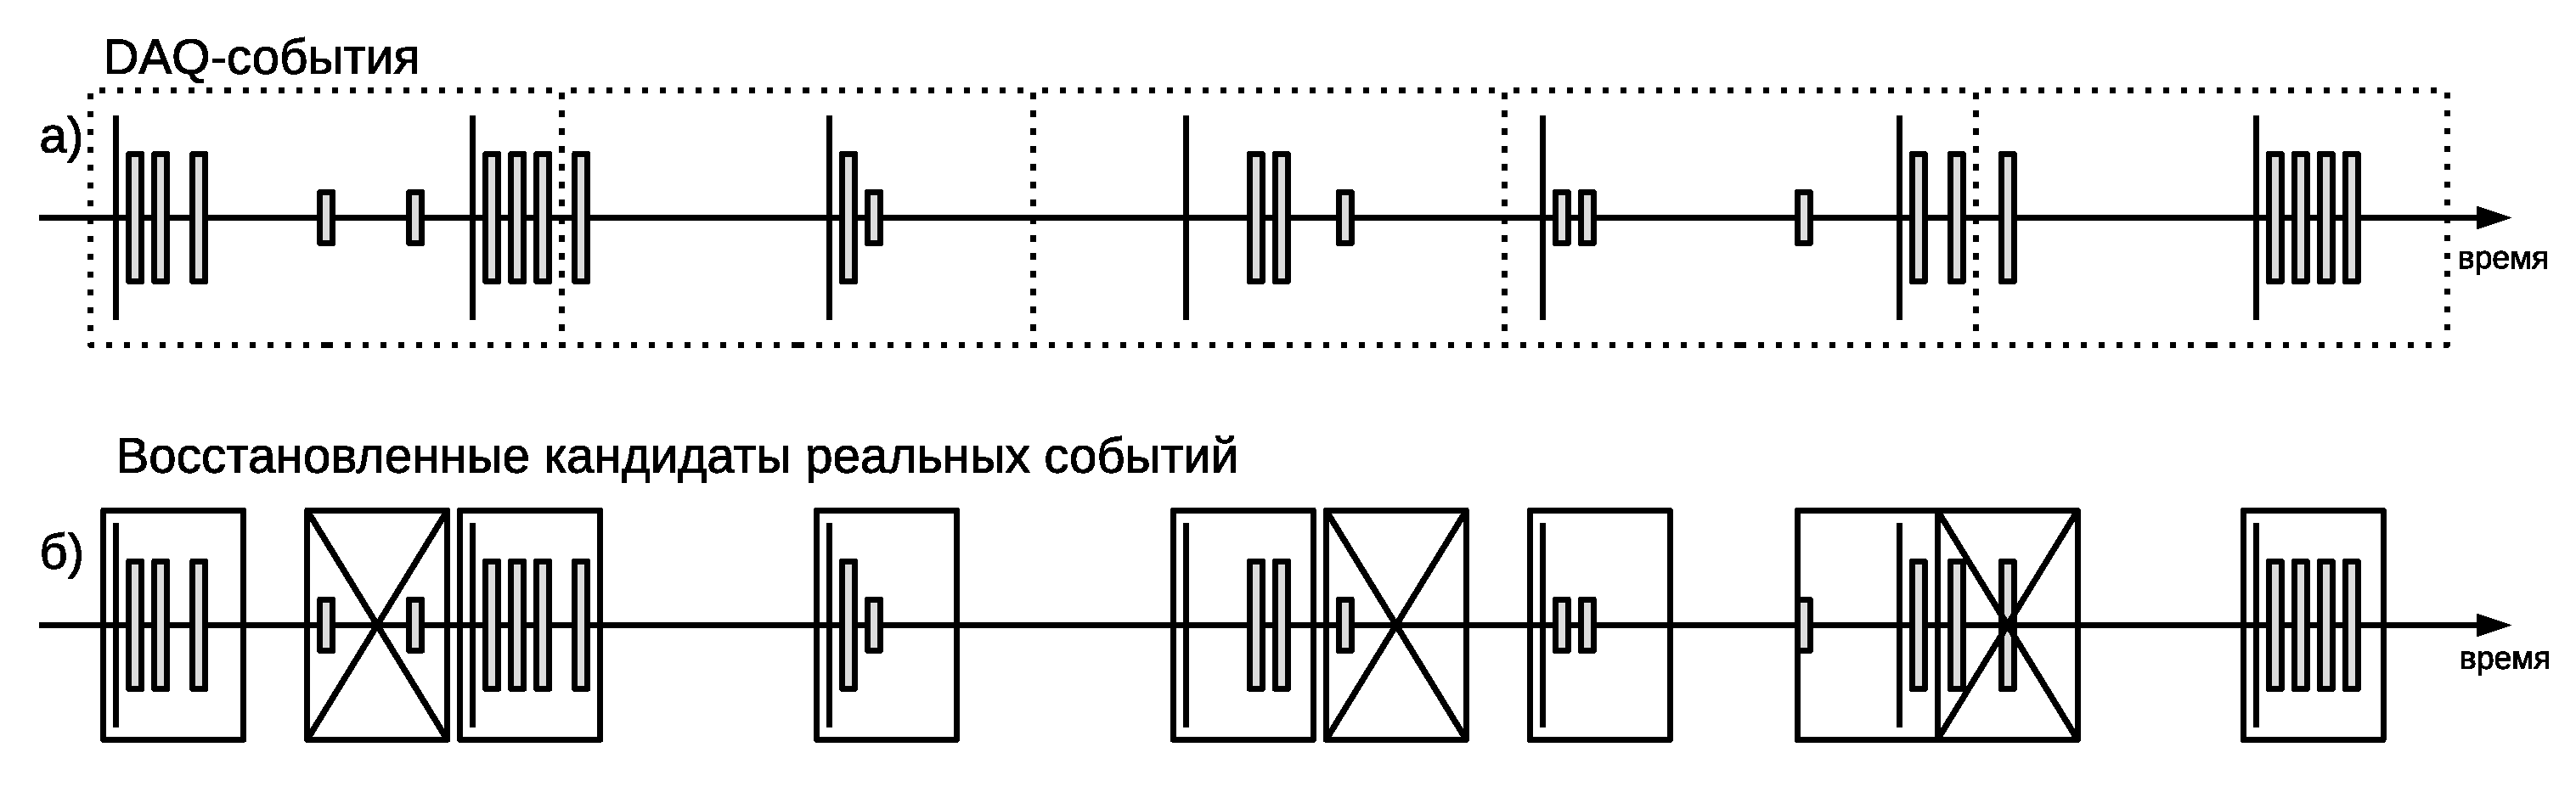
\includegraphics[width=1.0\textwidth]{pictures/15_Event_building_rus_bw.eps}
\caption{Идея алгоритма построения события: (а) поступающие данные, сгруппированные в DAQ-события; (б) востановленные кандидаты реальных событий; перечёркнуты отбрасываемые кандидаты, не содержащие триггер. Тонкие длинные линии --- триггерные сигналы, прямоугольники средней длины --- сигналы, связанные со светом, короткие прямоугольники --- шумовые сигналы.}
\label{fig:EventBuilding}
\end{figure}

Рассмотрим некоторый интервал времени, приведённый на \figref{fig:EventBuilding}, в течение которого поступают:
\begin{itemize}
\item {Триггерные сигналы --- импульсы с генератора, питающего лазер, либо сигналы с детекторов пучка;}
\item {Сигналы, скоррелированные с импульсами с генератора или детекторами пучка, т.е. связанные со светом;}
\item {Шумовые сигналы, распределённые равномерно во времени.}
\end{itemize}

Очевидно, что реальное событие может попасть на границу DAQ-событий, следовательно, необходимо при построении реальных событий учитывать несколько DAQ-событий. Также в силу особенностей электроники не гарантируется, что входная информация поступает упорядоченной во времени. Поэтому периодически случается, что хиты реального события, пришедшего по большей части в $i$-м DAQ-событии, обнаруживаются в $i+1$, реже $i+2$, и даже $i+3$ и последующих DAQ-событиях. Следовательно, требуется сначала распознать кластеры хитов в достаточно широком интервале времени --- потенциальные события, а затем по наличию заданного типа триггера выбрать реальные события, содержащие либо черенковские кольца, либо вспышки лазера.

Реализован данный алгоритм с помощью буфера хитов. По мере распаковки входных сообщений, построенные хиты заносятся в буфер. На каждой итерации осуществляется распознавание кандидатов событий в буфере и определяется их количество $N$. Когда $N$ достигает заданного минимального уровня, на каждой итерации, помимо приёма одного входного DAQ-события, осуществляется выброс выходного кандидата реального события. Так как одно DAQ-событие может содержать несколько кандидатов, буфер будет расти. Для того, чтобы избежать переполнения, устанавливается верхний предел. Когда $N$ достигает этого предела, осуществляется сброс событий на выход по принципу FIFO до заданного минимального уровня. На \figref{fig:Buffer} приведён отрывок диаграммы наполненности буфера по мере обработки входного потока. В данном примере были установлены следующие параметры: минимальное кол-во событий в буфере 200, максимальное --- 500. Отметим, что кол-во событий в буфере может превышать заданное максимальное значение, если в одном DAQ-событии содержится более одного реального события. По окончании входного потока содержимое буфера обрабатывается полностью и все распознанные события подаются на выход.

\begin{figure}[H]
\centering
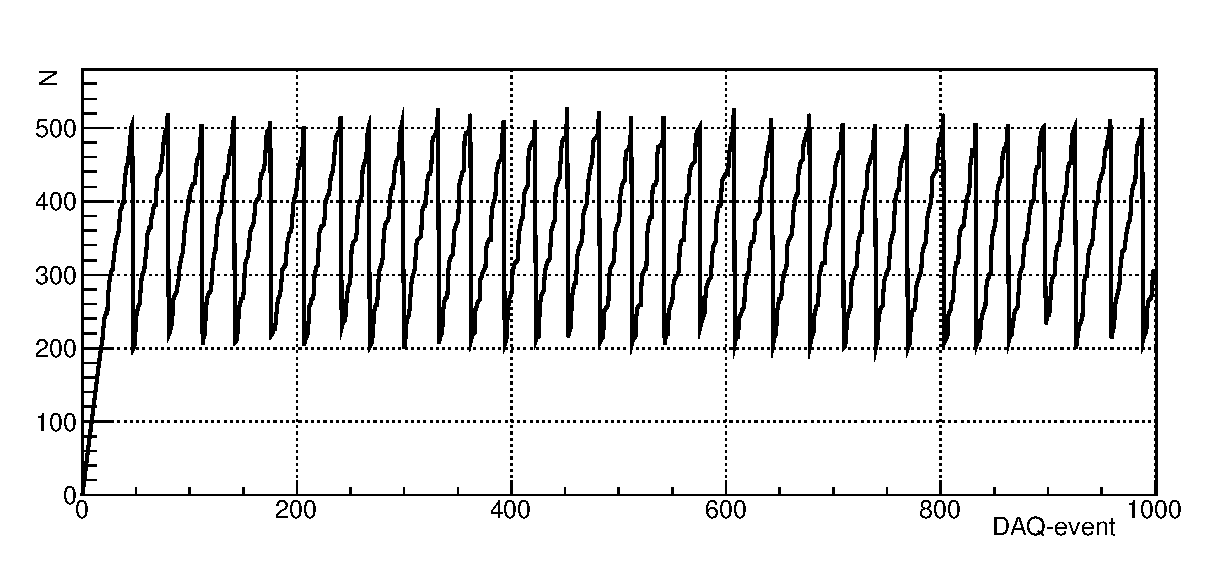
\includegraphics[width=1.0\textwidth]{pictures/16_Buff.eps}
\caption{Диаграмма наполненности буфера найденных событий в зависимости от номера обработанного входного DAQ-события.}
\label{fig:Buffer}
\end{figure}

\subsection{Реконструкция}\label{sec:secReconstruction}

Реконструкция в CBM~RICH означает поиск колец по хитам в плоскости реконструкции. В контексте реконструкции можно рассматривать хит как загоревшийся пиксель МА~ФЭУ. Конус черенковских фотонов, после фокусировки зеркалами, пересекает поверхность фоточувствительной камеры, которая в общем случае может состоять из нескольких плоскостей. Первый этап реконструкции --- перевод хитов из плоскостей камеры в плоскость реконструкции. Затем выполняется поиск колец по хитам. В CbmRoot есть реализации нескольких алгоритмов поиска колец. Наибольший практический интерес представляет алгоритм распознавания колец черенковского излучения, основанный на проеобразовании Хафа и описанный в работах~\cite{RECOPEPAN, RECO2}. Реализация данного алгоритма была специально адаптирована для данных пучковых тестов, в которых ожидается одно кольцо на событие. Данный алгоритм реализован в классе \classname{CbmRichProtRingFinderHoughImpl}, унаследованном от \classname{CbmRichProtRingFinderHough} и далее от \classname{CbmRichRingFinder}. После этого определяются параметры кольца и далее осуществляется реконструкция треков частиц с применением информации с других детекторов.
